\documentclass{report}
\usepackage[utf8]{inputenc}
\usepackage{xcolor}
\usepackage{url}
\usepackage[nottoc]{tocbibind}
\usepackage{graphicx}
\usepackage[bottom]{footmisc}
\usepackage{cite}
\usepackage{caption}
\usepackage{subcaption}
\bibliographystyle{ieeetr}

\title{Project Document: Deep(FAMS)}
\author{Mohammad Alyetama \\
Ali Al-Ramini \\
Fangyi Li }
\date{}

\begin{document}

\maketitle

\tableofcontents

\begin{abstract}
We present two project ideas that employ deep learning techniques. The first idea involves optimizing generative adversarial networks to generate good results with limited data using a recently proposed mechanism, the adaptive discriminator augmentation. The goal of this idea (Idea 1) is to evaluate the reproducibility and generalizability of the results generated by this proposed mechanism. \\The second idea requires using big cycling data to analyze the effect of temporal factors on bicycling. This project idea aims to create a model that correcting map cycling patterns in the State of Nebraska.
\end{abstract}

\chapter{Milestone 1: Project Ideas}

\section{Introduction}

\subsection{Project Idea 1}

Generative adversarial networks always seek to increase the dataset size to generate desirable results as an approach to generative modeling. The massive demand for data is challenging to lots of areas, and thus placing constraints on more widely being used of this practical approach. However, the dataset size reduction can cause overfitting issues in checking step by discriminator sub-model. Applying dataset augmentation can generate the augmented distribution, which is highly undesirable to generate samples.
An attempt to apply a wide range of augmentation by Kerras et al. is trying to demonstrate GAN can use a smaller dataset size but prevent the augmentation "leaking" at the same time. In this project, we will follow Karras et al. methods of adaptive discriminator augmentation mechanism~\cite{karras2020training} to try to reproduce their result.


\subsection{Project Idea 2}
There is a great interest in improving the cycling infrastructure in Nebraska by analyzing cyclic data. Toward this goal, we acquired the Strava Metro data covering Nebraska's state from January 2017 to December 2019.  Strava provides data into four categories edges, nodes, origin-destination polygons, and shapefiles that contain spatial attributes to create maps using GIS software. Edges are street segments between nodes. In other words, a set of edges form a street. Nodes are the intersections between edges, and origin-destination polygons divide a space into smaller areas. Every category of Strava data is divided into yearly, monthly, and hourly data. The Strava data, made available by the social fitness network company Strava, includes raw data for the hour-by-hour counts for bicycle trips that have been mostly incorporated into existing maps for better visualization. In this project, we propose building a deep learning regression model that utilizes Strava data in addition to weather data to predict the number of cycling trips in Nebraska. 

\section{Project Idea 1: Evaluating the Reproducibility of Training GAN With Limited Data}

Generative adversarial networks (GAN) is a generative modeling approach that uses deep learning techniques to automatically discover and learn the input patterns to generate an output that would plausibly appear as if it was sampled from the original input data~\cite{goodfellow2014generative}. For example, a GAN that uses convolutional neural networks (CNNs) can take pictures of humans as input data and generate new pictures of humans with plausible characteristics that look superficially genuine. This approach gained popularity after it was introduced by Goodfellow and his colleagues in 2014~\cite{goodfellow2014generative}. In their paper, they describe GAN as a structure with two essential sub-models: (1) a generator model that learns to generate superficially plausible data, which the discriminator takes as negative training examples, and (2) a discriminator model that learns to discriminate between generated and real data, and penalizes the generator if an implausible result is detected~\cite{creswell2018generative}. The generator and the discriminator are neural networks that are directly connected. This connection allows the discriminator to send a signal, through backpropagation, that the generator uses to update its weights. Specifically, the generator samples a vector that is randomly drawn from a Gaussian distribution and use it to seed its generative process and match it to a distribution of interest, creating a "latent space." With sufficient training, the generator model can learn the input data's statistical latent space and create output data similar to what is observed in the input data~\cite{radford2015unsupervised}. An example of such data is then processed by the discriminator model and attempt to distinguish it from the real distribution of the data (i.e., a binary class of fake/real). The generator model's goal here is to maximize the error of the discriminator model. In other words, the generator model becomes more effective the more the discriminator process fake data as real data. The GAN approach has been used in fashion, science, and video games with impressive results~\cite{gui2020review}.

However, a significant challenge in this area is the large number of data required to build a good GAN model, which is in some cases not available for researchers interested in applying GAN to their research question. GAN typically requires a large dataset because, with smaller datasets, the discriminator model ends up overfitting to training data examples, and the training eventually diverges~\cite{zhao2020improved}. While dataset augmentation is typically applied in such situations to solve overfitting~\cite{shorten2019survey}, it cannot achieve this in GAN models. The inability to solve this problem with dataset augmentation stems from GAN's ability to employ this technique without learning the augmented distribution and leaking these results to the model~\cite{zhao2020improved} causing undesirable outcomes. Therefore, the challenge is to demonstrate that GAN can be used with smaller datasets without the pitfalls mentioned above.

A recent attempt to solve this problem was proposed by Kerras et al.~\cite{karras2020training}, demonstrating that it is possible to obtain good results using limited data. The critical point in their proposed approach is that we can prevent overfitting and augmentations leak by applying a wide variety of augmentation methods. Their work demonstrates the validity of their approach by describing a set of conditions that allows controlling the augmentations leak problem and then proposes an adaptive discriminator augmentation pipeline that can dynamically control the strength of the augmentation. This is a novel approach they propose contrasting the convention of tuning the augmentation strength manually, a resources-consuming process. The process of building an adaptive discriminator augmentation mechanism, as described by the authors, is achieved by 
(a) Declare an overfitting heuristic, r, in which a value of zero represents no overfitting and a value of 1 means perfect overfitting.
(b) Adjust augmentation probability (\textit{p}) until the heuristic reaches a target value, which in turn can be processed by:
(1) initializing the augmentation strength to zero, then adjusting p every four mini-batches based on an overfitting heuristic (\textit{rf}).
(2) if \textit{rf} shows too much overfitting, it is countered by a fixed increment of \textit{p} (or fixed decrement if \textit{rf} shows too little overfitting).
(3) The adjustment size is then set in a way that allows p to quickly rise from 0 to 1 while clamping p after every step from below to zero (adaptive).
(4) The results from adaptive versus fixed \textit{p} are then compared.
Using such mechanisms on limited data, the authors demonstrated that their adaptive discriminator augmentation approach improved the quality of the result and stabilized training with a minimal effect on resources consumption, showing that their strategy is both viable and cost-efficient~\cite{karras2020training}.


In this project, we will attempt to reproduce the results reported by Karras et al. using their adaptive discriminator augmentation mechanism. We expect our reproduced work to support Kerras et al.'s claim made in the paper; that is, good results can be obtained in a GAN model with only a few thousand training images. The original article's hypothesis was tested using five small datasets (METFACES, BRECAHAD, AFHQ, and CIFAR-10). Here, we plan to test adaptive discriminator augmentation on additional datasets to find out whether the scope of Kerras et al. paper is generalizable. This would be a pivotal point in our project because the authors of the article claim that their model's strength stems from its ability to work despite variations between datasets in content and size. This is a central argument to their approach. They experimentally demonstrate that a set of fixed augmentation parameters (as opposed to adaptive parameters) will miss the utmost advantage a GAN model can achieve. Overall, our results will allow us to evaluate the reproducibility of the results, the readability of the source code, and experiment with the ability to generalize the approach described in the paper with different datasets.



\section{Project Idea 2: Using App Data to Model Bicycling Patterns in Nebraska}

Across the United States, cycling is becoming increasingly popular as users shift travel modes amid concerns of health, physical activity, air, and environmental quality, and to escape roadway congestion. Unfortunately, the infrastructure in the U.S. traditionally caters to automobile traffic creating impediments for bikers and impacting their safety. To accommodate cycling, a major challenge is the lack of machine learning model representation of the available data to assess the attributes of present assets accurately and to inform additional investments to integrate bicycles into our transportation system. Toward that end, this project uses citywide bicycle travel data (i.e., Strava Metro Data) to provide a comprehensive description of daily cycling in a mid-size American state as a proof-of-concept approach to planning for cycling. 
\\Various governments and organizations utilize big data to evaluate their cycling infrastructure ~\cite{hall2012open}. Big cycling data are usually collected using live point data, journey data, Bike-Share Programs (BSP), and GPS. Live point data are collected on intersections using cameras on traffic lights, counting stations, or even sensors. While the journey data provide information about the origin and the destination of the trip, it does not provide the trip details. This set of data could be collected from BSP or by other sources like online questionnaires. BSP data are complete and in real-time. However, these data only give information within the area of its location ~\cite{ romanillos2016big, rogers2000counting}. Strava is considered a GPS program that is made available by the social fitness network company Strava. Strava utilizes the Open Street Map (OSM) to deliver its data. These GPS data are very detailed and historical but represent a small sample of the cyclists' total population.  
Strava app data contains a vast amount of spatial and temporal details to predict cycling activity patterns. It provides a good approximation of the most-used routes and the peak months and hours. To protect privacy, the Strava data set is combined into population datasets. While a small portion of cyclic may use Strava to log their trips or the app might track trips for users using other transportation methods ~\cite{hall2012open, romanillos2016big, fishman2016cycling }, several studies showed that there is a strong correlation between the Strava data and the ground-truth data obtained from counting stations ~\cite{hong2020evaluation, jestico2016mapping}. 
Cycling is affected by several factors such as weather, time of the day, infrastructure, congestion, environment, income, public transportation, health, population density, the slope of the street, and cultural view towards cycling ~\cite{musakwa2016mapping, roy2019correcting, hochmair2019estimating}. But traditionally, access to high-quality data has limited our understanding of cycling behavior and route choice in the face of these myriad factors. In this project, we explore the weather effects and weather parameters sensitivity to cycling in Nebraska. This work aims to specify cycling behavior further as it relates to specific factors, but more importantly, to determine the quality of the specified factors in determining the number of cycling trips over a vast area like the State of Nebraska. 
Using data visualization techniques and Deep learning regression (e.g., ANN, RNN, LSTM, and GRU)~\cite{hassoun1995fundamentals, graves2013generating} we study the most influential time-related factors affecting the cycling patterns in Nebraska. Moreover, cycling is usually categorized into two classes, commuting and recreational. The proposed study will take advantage of the data shared by Strava to predict the number of commutes and recreational activities across all streets. 

\section{Conclusions}
\subsection{Project Idea 1}
The core of this project is to test if the methods proposed by Karras et al. can solve the problem of augmentation leak and then ease the burden of huge datasets required by GAN. Given that the proposed mechanism is relatively new and paradigm-shifting, we believe that the idea of reproducing the paper's results would be greatly valuable. Studying such an approach to solve overfitting and subsequent problems while using limited datasets in GAN allows any researcher access to cost-efficient models.

\subsection{Project Idea 2}
This project provides an exciting idea: to create a deep learning model that predicts Nebraska's cycling patterns. With the help of high-quality data sources (e.g., Strava Data and Weather Data), this project's outcomes could be essential towards understanding how cyclists react to temporal variations. However, the spatial factors affecting cycling should also be studied, adding more complexity to the problem. The spatial representation of the data could be tough to map during this short period. Additionally, this idea is essential considering the current situation with COVID-19, adding more complexity and difficulty to reproducing the analysis to agree with the latest status.

\chapter{Milestone 2: Project Selection}

%In this chapter, you should select your project, formally define it, and propose two approaches, each with a work plan.  You should follow the The Heilmeier Catechism~\cite{heilmeier}, which is a set of questions used to evaluate proposed research programs:  
%\begin{enumerate}
   % \item What are you trying to do? Articulate your objectives using absolutely no jargon.
   %\item How is it done today, and what are the limits of current practice?
   %\item What is new in your approach and why do you think it will be successful?
   %\item Who cares? If you are successful, what difference will it make?
   %\item What are the risks?
   %\item How much will it cost?
   %\item How long will it take?
   %\item What are the mid-term and final ``exams'' to check for success?
%\end{enumerate}

\section{Introduction}

Our group semester project is Evaluating the Reproducibility of Training GAN with Limited Data.
As mentioned in the last chapter, GAN, representing Generative Adversarial Networks, is a generative modeling approach using deep learning techniques to automatically discover and learn the input patterns to generate an output that would plausibly appear as it was sampled from the original dataset\cite{goodfellow2014generative}. The GAN approach has gained its popularity in diverse areas including but not limited to fashion, science, and video games\cite{gui2020review}. The success of GAN approach can be contributed to its structure: a generator model and discriminator model connecting together, where the generator model learns to generate superficially plausible data, and the discriminator model takes the generated data to discriminate with the real data and penalizes the generator if there’s an implausible result detected\cite{creswell2018generative}. The connection between two models allows the updating of generator based on the discrimination of discriminator, and generating the more plausible outputs\cite{radford2015unsupervised}. However, its success is still weakened by the challenge of its needs for the large dataset, to make sure the efficiency of the GAN approach. The applying of small dataset makes the discriminator ended up overfitting to training data examples, and the training diverged\cite{zhao2020improved}. What’s more, if the augmentation of dataset is simply introduced to resolve the overfitting, the augmented distribution can be caused, which is highly undesirable for sample generation.\cite{zhao2020improved} Therefore, it is a challenge that applying GAN approach with smaller dataset and avoid the mentioned pitfalls at the same time. In the research by Kerras et al\cite{karras2020training}, one method was come up to realize obtaining the good results using smaller dataset. The research was applying a wide variety of augmentation methods, and the results demonstrated the validity by describing a set of conditions that allows controlling the augmentations leak problem and then proposed an adaptive discriminator augmentation pipeline that can control the strength of the augmentation. 

The paper provides the possibility for small dataset to obtain good result from GAN approach; this possibility is valuable since the broke of dataset size limitation will help GAN approach spreading in more areas, and correspondingly those areas will obtain an efficient way to solve their problems. 
The offered methods are providing us the prospect for the future similar problems, which is a great chance for us to learn about model learning. Additionally, the decision on Evaluating the Reproducibility of Training GAN with Limited Data is also the result of considering the feasibility within the limited one-semester timeline: 
the small size of dataset won’t discourage us to start with, and the provided methods in paper did a good demonstration for reproducing and won’t take too much time to lag behind the timeline.


\section{Problem Specification}

%Formally define your chosen problem, including the following, as subsections:
%\begin{enumerate}
%    \item A brief statement of your project topic (HC1).
%    \item Motivation for your topic: why it is important and interesting (HC3, HC4). If your work is in an application area, be careful to avoid technical jargon from that area that is outside of computer science. If you must use a term, define it as carefully and simply as possible.
%   \item What resources will you need, including data sets and libraries that need to be installed on {\tt crane} (HC6).
%   \item Cite at least three references (at least two published journal or conference papers) (HC2).
%\end{enumerate}

The work presented in this project provides a complete evaluation of the proposed generative image training models by Karras et al in\cite{karras2020training}. The idea is to reproduce the generative image models trained on significantly fewer data compared to other approaches in the past. We are going to use the adaptive discriminator augmentation mechanism proposed in paper, following the codes provided in\cite{karras2020training}, to assess its reproducibility and ability to classify relatively small (few thousands) datasets.\\


In many application fields it is challenging to collect large datasets to perform data training. For example, in medicine there is an ongoing challenge in modeling possible appearance of biological specimens (tissues, tumors, etc.) This is a growing body of research that seems to constantly suffer from limited high-quality data. As introduced above, GAN has a great performance in training unlimited online data\cite{goodfellow2014generative, miyato2018cgans, miyato2018spectral, brock2018large, karras2017progressive, karras2019style, karras2020analyzing}, as a result it cannot be used for lots of specific applications that only collected around hundreds or thousands of samples, where collecting more samples can be very complicated and costly. If the small datasets are applied for GAN approach, the overfitting would occur in discriminator, and the dataset augmentation always used for overfitting can lead to training divergence in this GAN approach situation, which will not get a good result in the end. The method proposed by Kerras et al has been providing the chance to break this deadlock, to make GAN approach more suitable for small datasets, this method takes use of a wide range of augmentations to ensure that the discriminator does not overfit, while the generator does not also leak. The success of this method will make GAN approach more available for those specific applications with relative small datasets, where's a great potential to solve more problems. Thus, in this project we evaluate the GAN augmentations proposed by Karras et al and reproduce their approaches in terms of model architecture and code. Moreover, we test the model on several additional small datasets and compare our results with the results obtained by the original paper authors, to find out if the scope of the model is generalizable. From an applied point of view, this work contributes to efficiency; by testing the GAN augmentations proposed, this work will further confirm the elimination of the barrier for applying GAN-type
models in many applied fields of research. \\

In this project, there are some requirements mentioned in the original paper to make sure reproduce the study successfully:
\begin{itemize}
    \item 64-bit Python 3.6 or 3.7. Anaconda3 with numpy 1.14.3 or newer.
    \item TensorFlow 1.14, which was used for all experiments in original  paper, but TensorFlow 1.15 is also supported on Linux. If on Windows use TensorFlow 1.14.
    \item 1–8 high-end NVIDIA GPUs with at least 12 GB of GPU memory, NVIDIA drivers, CUDA 10.0 toolkit and cuDNN 7.5.
    \item On Windows, the compilation requires Microsoft Visual Studio to be in PATH. It is recommended to install  Visual Studio Community Edition and add it into PATH using "C:\Program Files (x86)\Microsoft Visual Studio\2019\Community\VC\Auxiliary\Build\vcvars64.bat".
\end{itemize}



we will use several datasets that consist of a limited number of training images, including: 
\begin{enumerate}
\item METFACES\cite{karras2020training} 
\item AFHQ\cite{choi2020stargan}
\item CIFAR-10\cite{krizhevsky2009learning}
\item StandfordDogs\cite{}
\item Cars196\cite{}
\item OxfordFlowers102\cite{}
\end{enumerate}


\section{Proposed Method:}

%%%%%%%%%%%%%%%%%%%%%%%%%%%%%%%%%%%%%%%%%
%Propose a step-by-step approach to solve your chosen problem.  You should include 
%a precise work plan: what you plan to do, what data sets you will test on, how you will preprocess the data, what the steps (pipeline) of this method (e.g., what NN architecture(s) will be used and how they'll be linked), how you will evaluate performance, what is your timeline, etc.\ (HC5, HC7, HC8).  One or more of your references should relate to aspects of this. 
%%%%%%%%%%%%%%%%%%%%%%%%%%%%%%%%%%%%%%

In this section, we provide details of the methods we plan to use in this paper.

\begin{itemize}
    \item \textbf{Datasets.} In our experiments, we will use three out of the six datasets used in the original paper. That is, {\tt METFACES}, the Animal Faces-HQ ({\tt AFHQ}) dataset, and {\tt CIFAR-10}. In addition to these three datasets, we will test the generalizability of the original paper's findings by using three other small datasets that were not tested in Kerras et al. paper. These are the {\tt StanfordDogs} dataset, the {\tt Cars196} dataset, and the {\tt OxfordFlowers102} dataset. See Table 1 for more details about the datasets we plan to use in the present project. The datasets wil be either downloaded from Tensorflow datasets collection (CIFAR-10, Cars196, OxfordFlowers102, and StanfordDogs) or from source (AFHQ and METFACES).
    
    \item \textbf{Preprocessing.} The {\tt METFACES} dataset is available in both raw and process format. We will use the raw format and process it by aligning and cropping images at 1024×1024 pixels, then use various automatic filters to prune the dataset. The {\tt AFHQ} dataset will be split into three subsets: CAT, DOG and WILD. All datasets will be standardized to make the training faster and to reduce the probability of getting stuck in a local optima.
    
    \item \textbf{Pipeline}.
    The authors of the paper implemented their techniques on top of the {\tt StyleGAN2} official TensorFlow implementation and kept most of the network architecture unchanged.  For this project, we will use  use the baseline StyleGAN2 as illustrated in Figure 1.
    \begin{enumerate}
        \item \textbf{\textit{The generator model.}} The generator model starts with an input layer that takes an image as input and a vector as an output in the latent space and gets normalized. We follow this with two fully connected layers (Dense layers), then we add a 4×4 convolutional layer, a 4×4 ToRGB layer, then an UpConv layer (upsampling + Sum + Residual Unit). We repeat this six more times while increasing the kernel size by the power of 2 (8×8, 16×16, 32×32, etc.). 
        
        \item \textbf{\textit{The discriminator model.}} For the discriminator model, following the input layer we will add a FromRGB layer with a kernel size of 256×256, followed by a DownConv layer (convolutional layer + Residual Unit + downsampling), a skip connections. We will repeat this 6 times before we add a a mini-batch standard deviation, a convolutional layer then a fully connected layer.
        
        \item \textbf{\textit{Quality metrics.}} In this project, we will use multiple metrics to evaluate the performance of our GANS.
        \begin{itemize}
            \item We will compute Frechet Inception Distance (FID) against the full dataset for each network to evaluate it.
            \item Then, we will compute the Kernel inception distance (KID) against the full dataset.
            \item Finally, we will calculate precision and recall againt the full dataset.
        \end{itemize}
        
    \end{enumerate}
    
    \item \textbf{\textit{Timeline.}} The project timeline is described in Figure 2.

\end{itemize}


\begin{table}[h]

        \centering 
        \caption{Datasets Information}
        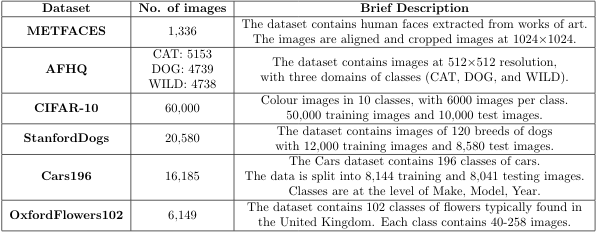
\includegraphics[width=\textwidth]{figs/table_1.png}
\end{table}


\begin{figure}[h]
    \centering 
    \caption{StyleGAN2 architecture}
    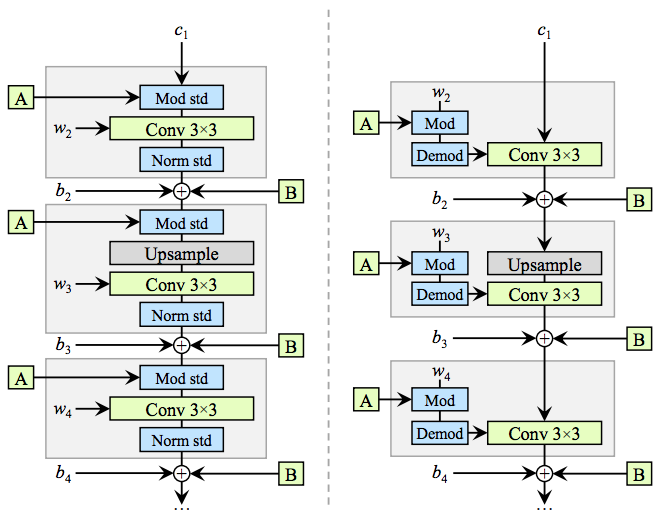
\includegraphics[width=\textwidth]{figs/stylegan2_arch.png}
\end{figure}

\begin{figure}[h]
    \centering 
    \caption{Project Timeline}
    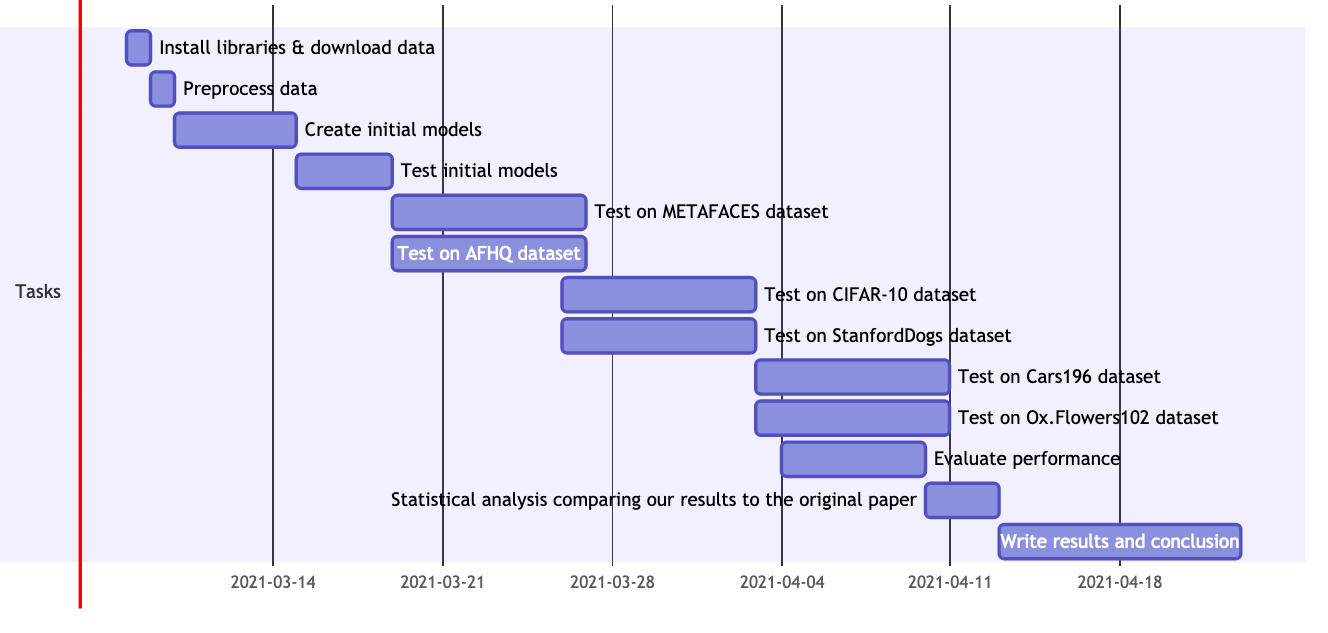
\includegraphics[width=\textwidth]{figs/timeline.png}
\end{figure}



\section{Conclusions}

%Sum up, including your opinion on each approach.  Also, list any questions that you have for the instructor and TA regarding your project work.
GAN approach is an efficient generative modeling approach, but its high demand of dataset size makes it limited to small size datasets applications. The attempts in Kerras et al provided a method to increase the feasibility of GAN approach for small size datasets. By the applying of adaptive discriminator augmentation mechanism, the GAN approach can also generate a good result with small datasets. In our project, we try to reproduce this good quality of results reported in paper, following the code of the method and applying them to small datasets (three from original paper, and three additional new datasets). As described above, after the preprocessing of data, we are going to follow the pipeline where the baseline is StyleGAN2.
The paper provides good details of method to allow us to reproduce the results. And we have confidence to follow the timeline we assumed within tiny error or not.


%\textcolor{red}{Remember to cite sources using BiBTeX and add those references to the end of this document!}

%It is okay to cite some websites and tutorials (if you first look up how to properly cite them!), but you must also cite some refereed publications from conferences and/or journals.




\bibliographystyle{plainurl}
\bibliography{main}

\end{document}
